\documentclass[14pt]{extarticle}  
\usepackage[T2A]{fontenc}  
\usepackage[utf8]{inputenc}
\usepackage[russian, english]{babel}
\usepackage{times}  
\usepackage{geometry}
\usepackage{listings}
\usepackage{xcolor} 
\usepackage{graphicx}
\usepackage{float}
\usepackage{caption}
\usepackage{gatherenum}
\usepackage{url}


\lstset{
	basicstyle=\ttfamily\footnotesize,
	keywordstyle=\color{blue}\bfseries, % Стиль ключевых слов
	commentstyle=\color{gray}\itshape, % Стиль комментариев
	stringstyle=\color{red}, % Стиль строк
	numbers=left, % Включение номеров строк
	numberstyle=\tiny\color{gray}, % Стиль номеров строк
	stepnumber=1, % Шаг номеров строк
	numbersep=5pt, % Отступ номеров строк
	backgroundcolor=\color{white}, % Цвет фона
	showspaces=false, % Показ пробелов
	showstringspaces=false, % Показ пробелов в строках
	showtabs=false, % Показ табуляций
	tabsize=2, % Размер табуляции
	captionpos=b, % Позиция подписи
	breaklines=true, % Перенос длинных строк
	breakatwhitespace=false, % Перенос по пробелам
	escapeinside={\%*}{*)}, % Экранирование текста
	morekeywords={*,...} % Дополнительные ключевые слова
}

\geometry{a4paper, left=2cm, right=2cm, top=2cm, bottom=2cm}
\begin{document}

\thispagestyle{empty}
\begin{titlepage}
	\begin{center}
		\textbf{Министерство науки и высшего образования Российской Федерации}\\
		\textbf{ФЕДЕРАЛЬНОЕ ГОСУДАРСТВЕННОЕ АВТОНОМНОЕ ОБРАЗОВАТЕЛЬНОЕ УЧРЕЖДЕНИЕ ВЫСШЕГО ОБРАЗОВАНИЯ НАЦИОНАЛЬНЫЙ ИССЛЕДОВАТЕЛЬСКИЙ УНИВЕРСИТЕТ ИТМО}
	\end{center}
	
	\vspace{2cm}
	
	\begin{center}
		\textbf{\Large Лабораторная работа №1}\\
		\textbf{\Large по дисциплине}\\
		\textbf{\Large “Линейная алгебра и анализ данных”}
	\end{center}
	
	\vspace{1cm}
	
	\begin{center}
		\textbf{\Large Семестр I}
	\end{center}
	
	\vspace{3cm}
	
	\begin{flushright}
		\begin{tabular}{r}
			\textbf{Выполнили:} \\
			студенты \\
			\\
			Тиганов Вадим Игоревич \\
			гр. J3112 \\
			ИСУ 467701 \\
			\\
			Вагин Арсений Антонович\\
			гр. J3112 \\
			ИСУ 465339\\
			\\
			\textbf{Отчет сдан:} \\
			XX.12.2024
		\end{tabular}
	\end{flushright}
	
	\vspace{3cm}
	
	\begin{center}
		Санкт-Петербург \\
		2024
	\end{center}
\end{titlepage}

\newpage
\pagenumbering{arabic}

\section*{Цель лабораторной работы}
Освоить основные концепции линейной алгебры и анализа данных по работе с матрицами. Научиться реализовывать и тестировать алгоритмы работы с матрицами в разреженно-строчном формате. Изучить и понять принципы работы алгоритмов, а также .tex верстания для создания отчета.



\vspace{0.5cm}

\section*{Задачи лабораторной работы}
\begin{enumerate}
	\item 
	\item 
	\item 
\end{enumerate}

\newpage
\section*{Ход выполнения лабораторной работы\\}
\begin{Large} 
	\textbf{Задача 1}\\
	
	 \end{Large} 
Задача заключалась в реализации следующих функий в классе: (был выбран ЯП Python, полный листинг кода см. в приложении А)
\begin{itemize}
	\item Ввод матрицы заданного размера пользователем.
	\item Подсчет следа матрицы.
	\item Поиск и вывод элемента матрицы по заданным индексам.
	\item Тестирование работы программы и создание консольного пользовательского интерфейса.\\
\end{itemize}

\begin{large}
	Использованные библиотеки и инструменты языка\\
\end{large}
В ходе написания программы были использованы только стандартные средства языка. Также для удобства и лучшей читаемости кода была импортирована библиотека typing.\\

\begin{large}
	Реализация функций и основные идеи\\
\end{large}
Все функции были реализованы в классе MatrixKeeper\\\\
Написаны функции:\\
inputMatrix - ввод матрицы пользователем,\\
trace - поиск следа матрицы,\\
findByIndex - поиск элемента по введенному индексу.\\

Суть работы алгоритмов:
\begin{itemize}
	\item inputMatrix: Приглашение пользователя ко вводу. Вначале через пробел вводятся два числа типа int - размер матрицы. Вторым приглашением вводится матрица по строке, элементы в строке разделяются пробелом.
	\item trace: След матрицы - сумма элементов главной диагонали этой матрицы. Циклом, оставаясь в пределах матрицы, проходимся по элементам с индексами вида [i][i], считаем сумму таких элементов. Можем так делать по той причине, что матрица имеет следующую структуру в классе:\vspace{3cm}
	\begin{lstlisting} [language=Python]
		self.matrix: Optional[List[List[float]]]
		\end{lstlisting} - то есть храним матрицу как список, каждый элемент которого является тоже списком.
	\item findByIndex: возвращаем элемент из матрицы, отнимая от индексов по единице, т.к. в ЯП отсчет начинается с нуля.
	\begin{lstlisting}
		return self.matrix[n-1][m-1]
	\end{lstlisting}
\end{itemize}
\begin{large}
	Тестирование программы\\
\end{large}
Написаны юниттесты для каждой функции класса с помощью стандартной библиотеки unittest. Также протестировано вручную.\\
Листинг кода теста см. в приложении А-test.\\
\begin{figure}[H]
	\centering
	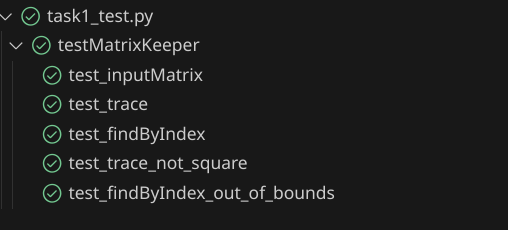
\includegraphics[width=0.5\linewidth]{tests-task1}
	\caption*{Успешное прохождение unittests}
	\label{fig:tests-task1}
\end{figure}
\begin{figure}[H]
	\centering
	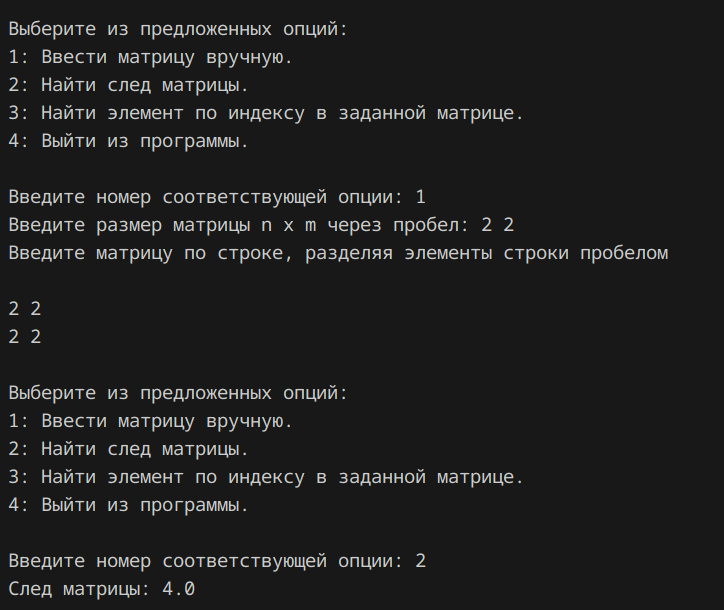
\includegraphics[width=0.5\linewidth]{tests-task2}
	\caption*{Ручной тест поиска следа матрицы 2х2 со всеми элементами, равными 2.}
	\label{fig:tests-task2}
\end{figure}
\begin{figure}[H]
	\centering
	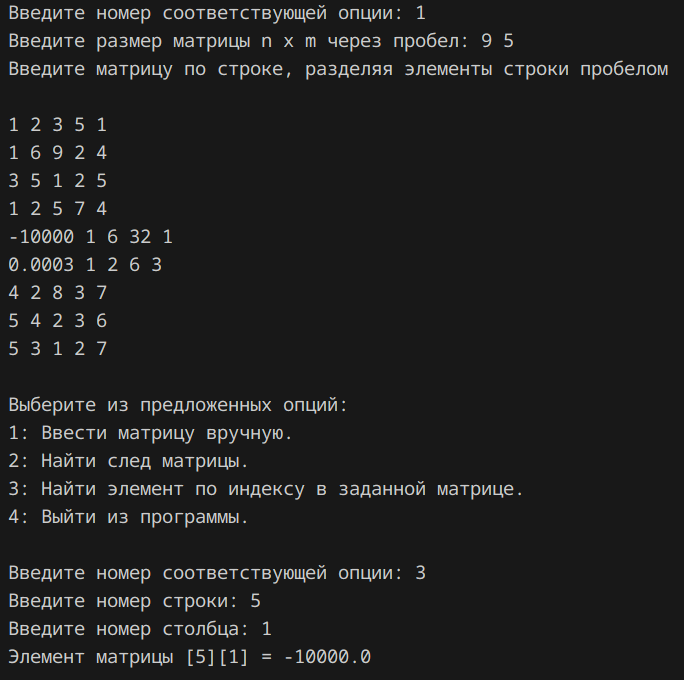
\includegraphics[width=0.5\linewidth]{tests-task3}
	\caption*{Ручной тест поиска страшного элемента в страшной матрице 9х5.}
	\label{fig:tests-task3}
\end{figure}
Итак, справились с первым заданием.\vspace{2cm}

\begin{large}
	Задача 2\\
\end{large}
Во второй задаче требуется реализовать три функции для операций с матрицами: (полный листинг кода см. в приложении Б)\\
\begin{itemize}
	\item Сложение двух матриц.
	\item Умножение двух матриц.
	\item Умножение матрицы на скаляр.\\
\end{itemize}

\begin{large}
	Использованные библиотеки и инструменты языка\\
\end{large}
В ходе написания программы были использованы только стандартные средства языка. Также для удобства и лучшей читаемости кода была импортирована библиотека typing.\\\\
Были реализованы 3 функции:\\
matrixAddition - сложение двух матриц.\\
matrixByMatrixMultiplication - перемножение двух матриц.\\
matrixScalarMultiplication - умножение одной из двух матриц на заданное число.\\
Согласно техническому заданию, функция ввода матрицы пользователем была импортирована из файла предыдущего задания. (inputMatrix)

Суть работы алгоритмов:
\begin{itemize}
	\item \textbf{matrixAddition}: Классическое сложение матрицы. Возвращаем матрицу, где каждый элемент с определенными индексами равен сумме элементов с соответствующими индексами из складываемых матриц.
	\begin{gather*}
		(A+B)_{i,k} = A_{i,k} + B_{i,k}
	\end{gather*}
	
	\item \textbf{matrixByMatrixMultiplication}: Умножение матрицы на матрицу. Возвращаем матрицу, где каждый элемент с определенными индексами равен сумме произведений элементов соответствующей строки первой матрицы и столбца второй матрицы.
	\begin{gather*}
		(AB)_{i,j} = \sum_{k=1}^{n} A_{i,k} \cdot B_{k,j}
	\end{gather*}
	
	\item \textbf{matrixScalarMultiplication}: Умножение матрицы на скаляр. Возвращаем матрицу, где каждый элемент равен произведению соответствующего элемента исходной матрицы и скаляра.
	\begin{gather*}
		(cA)_{i,j} = c \cdot A_{i,j}
	\end{gather*}
\end{itemize}
\begin{large}
	Тестирование программы\\
\end{large}
Написаны юниттесты для каждой функции класса с помощью стандартной библиотеки unittest. Также протестировано вручную.\\
Листинг кода теста см. в приложении Б-test.\\
\begin{figure}[H]
	\centering
	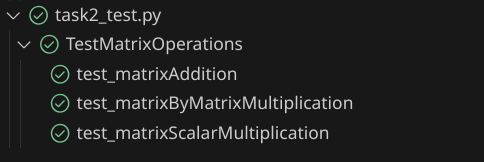
\includegraphics[width=0.5\linewidth]{tests-task4}
	\caption*{Успешное прохождение unittests}
	\label{fig:tests-task4}
\end{figure}
\begin{figure}[H]
	\centering
	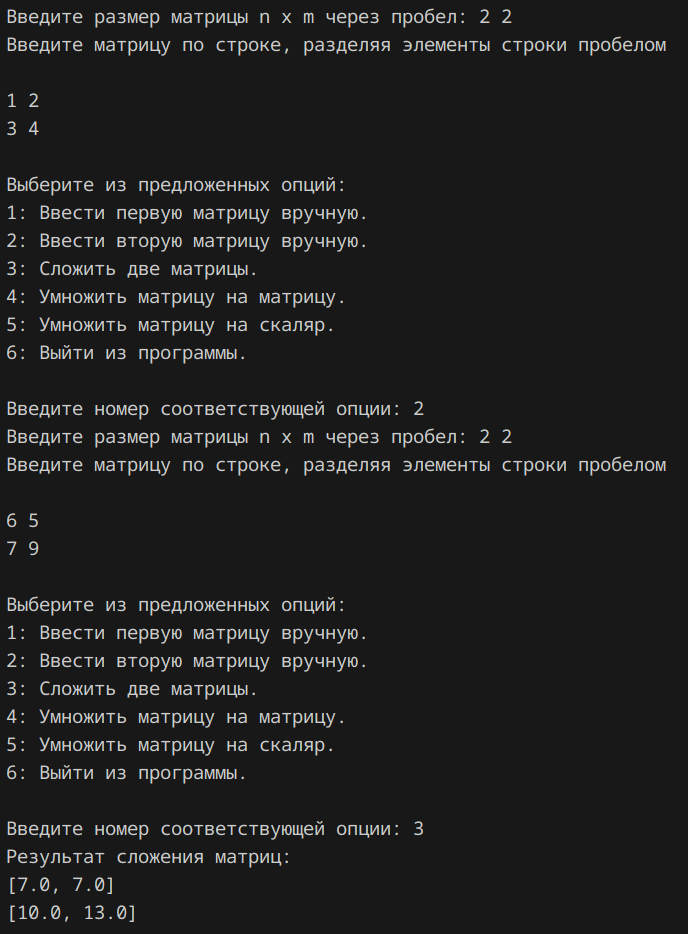
\includegraphics[width=0.46\linewidth]{tests-task5}
	\caption*{Ручной тест сложения двух матриц 2 на 2.}
	\label{fig:tests-task5}
\end{figure}
\begin{figure}[H]
	\centering
	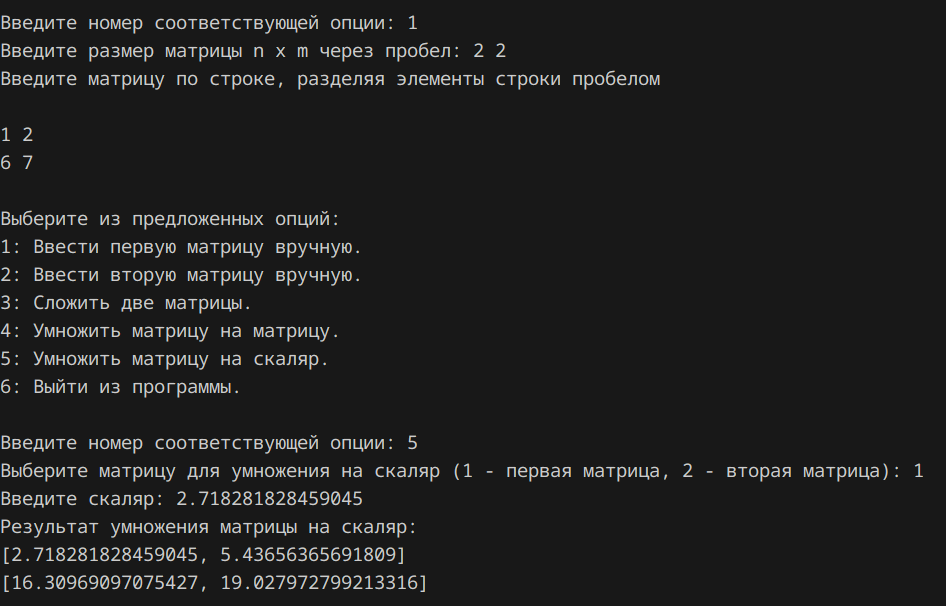
\includegraphics[width=0.58\linewidth]{tests-task6}
	\caption*{Ручной тест умножения матрицы 2 на 2 на число Эйлера с небольшим количеством знаков после запятой.}
	\label{fig:tests-task6}
\end{figure}
\begin{figure}[H]
	\centering
	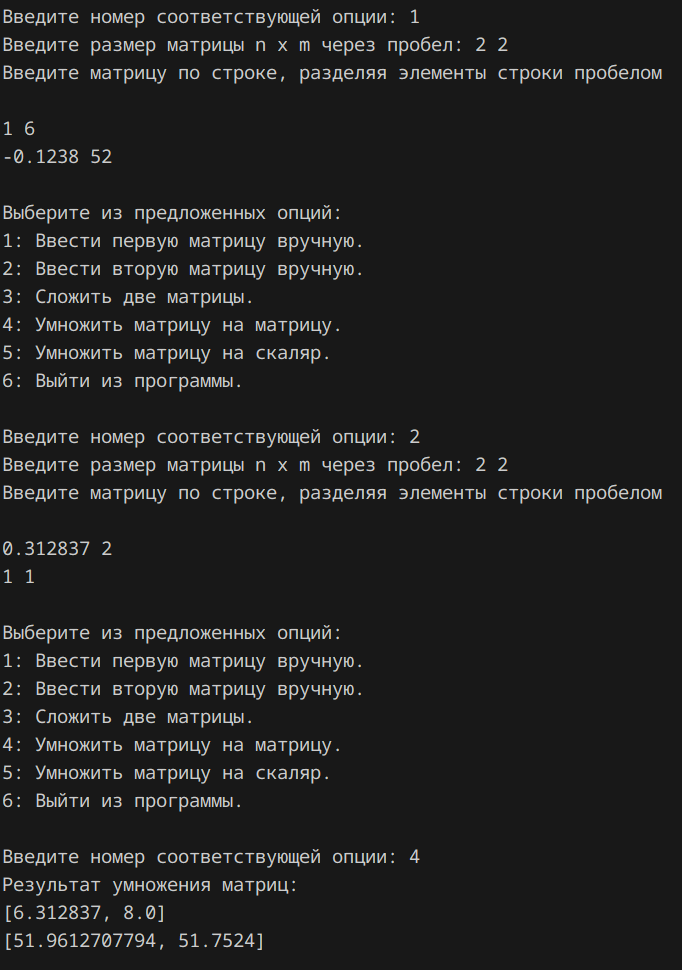
\includegraphics[width=0.7\linewidth]{tests-task7}
	\caption*{Ручной тест умножения двух страшных матриц 2 на 2.}
	\label{fig:tests-task7}
\end{figure}
\begin{figure}[H]
	\centering
	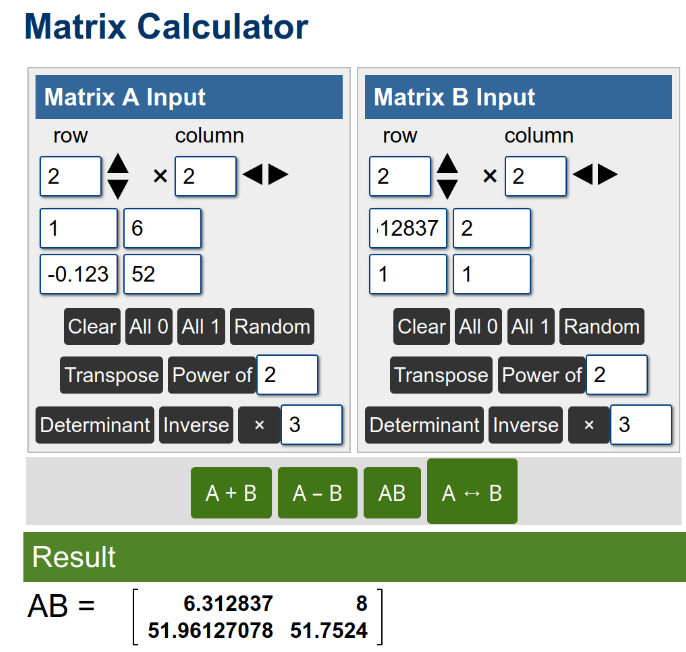
\includegraphics[width=0.5\linewidth]{tests-task8}
	\caption*{Удостоверимся в правильности полученного результата, умножив матрицы на сайте-калькуляторе. Результат правильный.}
	\label{fig:tests-task8}
\end{figure}
Справились со вторым заданием. \vspace{2cm}

\begin{large}
	Задача 3\\
\end{large}
В третьей задача требуется реализовать следующие функции: (полный листинг кода см. в приложении В)
\begin{itemize}
	\item Вычисление определителя матрицы. По тз - матрицы размером до 100х100
	\item Ответ на вопрос: существует ли матрица, обратная данной.
\end{itemize}


	
	
\newpage
\section*{Вывод}
\paragraph{}
В ходе выполнения данной работы были реализованы и протестированы различные функции для работы с матрицами. Это включало ввод матрицы, вычисление её следа, поиск элементов по индексам, а также операции сложения, умножения матриц и умножения матрицы на скаляр. Кроме того, были реализованы функции для вычисления определителя матрицы и проверки её обратимости.

Работа над этими задачами позволила нам углубить понимание основ линейной алгебры и её применения в программировании. Особенно интересным оказался метод Гаусса для вычисления определителя матрицы, который\\ демонстрирует применение алгоритмов линейной алгебры в решении сложных задач.

Процесс тестирования, как автоматического, так и ручного, подтвердил корректность реализованных алгоритмов и их способность работать с матрицами различных размеров. Это важно для обеспечения надежности и точности вычислений, что является важным аспектом в машинном обучении и анализе данных.

В целом, выполнение данной работы не только укрепило наши навыки программирования и работы с матрицами, но и заставило задуматься, как полученные знания помогут в будущем. Линейная алгебра является основой для многих алгоритмов машинного обучения, и понимание её принципов и методов является ключом для успешного применения этих алгоритмов на практике.

В будущем мы планируем продолжить изучение машинного обучения, включая более сложные алгоритмы и методы. Уверены, что полученные знания и навыки станут основой для дальнейшего развития в этой области.

\newpage
\section*{Приложения}
Пришлось все перевести на английский. Не понял, как в "lstlisting" в \LaTeX \ позволить писать русскими буквами без ошибок компиляции.\\ \\
\centering\begin{large}
	{Приложение А.\\
		 Полный листинг кода к первому заданию}\\
\end{large}

\begin{lstlisting}
	from typing import List, Optional
	
	class MatrixKeeper:
		def __init__(self):
			self.matrix: Optional[List[List[float]]] = None
		
		def inputMatrix(self) -> None:
		"""Input matrix
		First prompt - input matrix size n X m
		Second prompt - input the matrix row by row, elements separated by space"""
		
			try:
				n, m = map(int, input("Enter the matrix size n x m separated by space: ").split())
				self.matrix = []
				print("Enter the matrix row by row, separating elements with space\n")
				for _ in range(n):
					row = list(map(float, input().split()))
					if len(row) != m:
						raise ValueError("The number of elements in the row does not match m.")
						self.matrix.append(row)
			except ValueError as e:
				print(f"Input error: {e}")
				self.matrix = None
		
		def trace(self) -> float:
		"""Find the trace of the matrix"""
		
			if self.matrix is None:
				raise ValueError("Matrix has not been entered.")
			
			if len(self.matrix) != len(self.matrix[0]):
				raise ValueError("The matrix must be square to calculate the trace.")
		
		return sum(self.matrix[i][i] for i in range(len(self.matrix)))
		
		def findByIndex(self, n: int, m: int) -> float:
			"""Finds an element in the matrix by index n, m and outputs it"""
		
			if self.matrix is None:
				raise ValueError("Matrix has not been entered.")
		
			if n <= 0 or m <= 0 or n > len(self.matrix) or m > len(self.matrix[0]):
				raise IndexError("Indexes are out of the matrix bounds.")
		
			return self.matrix[n-1][m-1]
		
	def main():
		matrix_keeper = MatrixKeeper()
		
		while True:
			print("\nChoose from the following options:")
			print("1: Enter the matrix manually.")
			print("2: Find the trace of the matrix.")
			print("3: Find an element by index in the given matrix.")
			print("4: Exit the program.\n")
			
			try:
				option = int(input("Enter the number of the corresponding option: "))
				except ValueError:
				print("Incorrect input. Please enter a number.\n")
				continue
				
				if option == 1:
					matrix_keeper.inputMatrix()
				elif option == 2:
				try:
					trace_value = matrix_keeper.trace()
					print(f"Trace of the matrix: {trace_value}\n")
				except ValueError as e:
					print(e)
				elif option == 3:
					try:
						n = int(input("Enter the row number: "))
						m = int(input("Enter the column number: "))
						element = matrix_keeper.findByIndex(n, m)
						print(f"Matrix element [{n}][{m}] = {element}\n")
					except (ValueError, IndexError) as e:
					print(e)
				elif option == 4:
					print("Exiting the program.\n")
					break
				else:
					print("Incorrect input. Please choose an option from 1 to 4.\n")
	
	if __name__ == "__main__":
	main()
	
\end{lstlisting}

\centering\begin{large}
	{Приложение А-test.\\
		Полный листинг кода к тестам первого задания}\\
\end{large}
\begin{lstlisting}
	import unittest
	
	from codefiles.task1 import MatrixKeeper
	
	class testMatrixKeeper(unittest.TestCase):
	
		def setUp(self):
			self.keeper = MatrixKeeper()
		
		def test_inputMatrix(self):
		
			self.keeper.matrix = [
			[1.32, 2.32, 3.45],
			[2.1, 4.312, 4.24],
			[3.1, 1.12, 9.125]
			]
			
			self.assertEqual(self.keeper.matrix, [
			[1.32, 2.32, 3.45],
			[2.1, 4.312, 4.24],
			[3.1, 1.12, 9.125]
			])
			
			
		def test_trace(self):
		
			self.keeper.matrix = [
			[1.32, 2.32, 3.45],
			[2.1, 4.312, 4.24],
			[3.1, 1.12, 9.125]
			]
			
			self.assertEqual(self.keeper.trace(), 14.757)
		
		def test_findByIndex(self):
			
			self.keeper.matrix = [
			[1.0, 2.0, 3.0],
			[4.0, 5.0, 6.0],
			[7.0, 8.0, 9.0]
			]
			self.assertEqual(self.keeper.findByIndex(1, 1), 1.0)
			self.assertEqual(self.keeper.findByIndex(2, 2), 5.0)
			self.assertEqual(self.keeper.findByIndex(3, 3), 9.0)
		
		def test_trace_not_square(self):
		
			self.keeper.matrix = [
			[1.0, 2.0, 3.0],
			[4.0, 5.0, 6.0]
			]
			with self.assertRaises(ValueError):
			self.keeper.trace()
		
		def test_findByIndex_out_of_bounds(self):
		
			self.keeper.matrix = [
			[1.0, 2.0, 3.0],
			[4.0, 5.0, 6.0],
			[7.0, 8.0, 9.0]
			]
			with self.assertRaises(IndexError):
			self.keeper.findByIndex(4, 4)
\end{lstlisting}

\centering\begin{large}
	{Приложение Б.\\
		Полный листинг кода ко второму заданию}\\
\end{large}
\begin{lstlisting}
	from typing import List, Optional
	from codefiles.task1 import MatrixKeeper
	
	def matrixAddition(matrix_keeper1: MatrixKeeper, matrix_keeper2: MatrixKeeper) -> Optional[List[List[float]]]:
	"""Addition of two matrices"""
	
		if matrix_keeper1.matrix is None or matrix_keeper2.matrix is None:
			raise ValueError("One or both matrices have not been entered.")
		
		if len(matrix_keeper1.matrix) != len(matrix_keeper2.matrix) or len(matrix_keeper1.matrix[0]) != len(matrix_keeper2.matrix[0]):
			raise ValueError("Matrices must be of the same size for addition.")
		
		result = []
		for i in range(len(matrix_keeper1.matrix)):
			row = []
			for j in range(len(matrix_keeper1.matrix[0])):
				row.append(matrix_keeper1.matrix[i][j] + matrix_keeper2.matrix[i][j])
				result.append(row)
		
		return result
	
	def matrixByMatrixMultiplication(matrix_keeper1: MatrixKeeper, matrix_keeper2: MatrixKeeper) -> Optional[List[List[float]]]:
	"""Matrix by matrix multiplication"""
	
		if matrix_keeper1.matrix is None or matrix_keeper2.matrix is None:
			raise ValueError("One or both matrices have not been entered.")
		
		if len(matrix_keeper1.matrix[0]) != len(matrix_keeper2.matrix):
			raise ValueError("The number of columns in the first matrix must be equal to the number of rows in the second matrix.")
		
		result = [[0 for _ in range(len(matrix_keeper2.matrix[0]))] for _ in range(len(matrix_keeper1.matrix))]
		for i in range(len(matrix_keeper1.matrix)):
			for j in range(len(matrix_keeper2.matrix[0])):
				for k in range(len(matrix_keeper2.matrix)):
					result[i][j] += matrix_keeper1.matrix[i][k] * matrix_keeper2.matrix[k][j]
		
		return result
	
	def matrixScalarMultiplication(matrix_keeper: MatrixKeeper, scalar: float) -> Optional[List[List[float]]]:
	"""Matrix by scalar multiplication"""
	
		if matrix_keeper.matrix is None:
			raise ValueError("Matrix has not been entered.")
			result = []
		for row in matrix_keeper.matrix:
			result.append([element * scalar for element in row])
		
		return result
		
	def main():
		matrix_keeper1 = MatrixKeeper()
		matrix_keeper2 = MatrixKeeper()
		
		while True:
			print("\nChoose from the following options:")
			print("1: Enter the first matrix manually.")
			print("2: Enter the second matrix manually.")
			print("3: Add two matrices.")
			print("4: Multiply matrix by matrix.")
			print("5: Multiply matrix by scalar.")
			print("6: Exit the program.\n")
			
			try:
				option = int(input("Enter the number of the corresponding option: "))
				except ValueError:
				print("Incorrect input. Please enter a number.\n")
				continue
				
				if option == 1:
					matrix_keeper1.inputMatrix()
				elif option == 2:
					matrix_keeper2.inputMatrix()
				elif option == 3:
					try:
					result = matrixAddition(matrix_keeper1, matrix_keeper2)
					print("Result of matrix addition:")
					for row in result:
					print(row)
					except ValueError as e:
					print(e)
				elif option == 4:
					try:
						result = matrixByMatrixMultiplication(matrix_keeper1, matrix_keeper2)
						print("Result of matrix multiplication:")
						for row in result:
						print(row)
						except ValueError as e:
						print(e)
				elif option == 5:
					try:
						matrix_choice = int(input("Choose the matrix to multiply by scalar (1 - first matrix, 2 - second matrix): "))
						if matrix_choice == 1:
							matrix_keeper = matrix_keeper1
						elif matrix_choice == 2:
							matrix_keeper = matrix_keeper2
						else:
							raise ValueError("Incorrect matrix choice.")
						
						scalar = float(input("Enter the scalar: "))
						result = matrixScalarMultiplication(matrix_keeper, scalar)
						print("Result of matrix by scalar multiplication:")
						for row in result:
							print(row)
					except ValueError as e:
						print(e)
				elif option == 6:
					print("Exiting the program.\n")
					break
				else:
					print("Incorrect input. Please choose an option from 1 to 6.\n")
	
	if __name__ == "__main__":
	main()
\end{lstlisting}

\centering\begin{large}
	{Приложение Б-test.\\
		Полный листинг кода к тестам второго задания}\\ \\
\end{large}

\begin{lstlisting}
import unittest
from codefiles.task2 import matrixAddition, matrixByMatrixMultiplication, matrixScalarMultiplication
from codefiles.task1 import MatrixKeeper

class TestMatrixOperations(unittest.TestCase):

	def setUp(self):

		self.matrix_keeper1 = MatrixKeeper()
		self.matrix_keeper2 = MatrixKeeper()
		
		self.matrix_keeper1.matrix = [
		[1, 2, 3],
		[4, 5, 6],
		[7, 8, 9]
		]
		
		self.matrix_keeper2.matrix = [
		[9, 8, 7],
		[6, 5, 4],
		[3, 2, 1]
		]
	
	def test_matrixAddition(self):
		result = matrixAddition(self.matrix_keeper1, self.matrix_keeper2)
		expected = [
		[10, 10, 10],
		[10, 10, 10],
		[10, 10, 10]
		]
	self.assertEqual(result, expected)
	
	def test_matrixByMatrixMultiplication(self):
	
		self.matrix_keeper1.matrix = [
		[1, 2, 3],
		[4, 5, 6],
		[7, 8, 9]
		]
		
		self.matrix_keeper2.matrix = [
		[9, 8],
		[7, 6],
		[5, 4]
		]
		
		result = matrixByMatrixMultiplication(self.matrix_keeper1, self.matrix_keeper2)
		expected = [
		[38, 32],
		[101, 86],
		[164, 140]
		]
		self.assertEqual(result, expected)
	
	def test_matrixScalarMultiplication(self):
		scalar = 2
		result = matrixScalarMultiplication(self.matrix_keeper1, scalar)
		expected = [
		[2, 4, 6],
		[8, 10, 12],
		[14, 16, 18]
		]
		self.assertEqual(result, expected)

if __name__ == '__main__':
unittest.main()

\end{lstlisting}

\centering\begin{large}
	{Приложение В.\\
		Полный листинг кода к третьему заданию}\\ \\
\end{large}
 \begin{lstlisting}
 from task1 import MatrixKeeper
 from typing import List
 
 def determinantOfMatrix(matrix_keeper: MatrixKeeper) -> float:
 """Calculates the determinant of a matrix. Matrix size: up to 100x100."""
	 if matrix_keeper.matrix is None:
		 raise ValueError("Matrix is not defined.")
	 
	 matrix = matrix_keeper.matrix
	 if len(matrix) != len(matrix[0]):
		 raise ValueError("Determinant can only be calculated for a square matrix.")
	 
	 return gauss(matrix)
	 
 def isMatrixInvertable(matrix_keeper: MatrixKeeper) -> bool:
 """Checks if the inverse matrix exists (detA != 0)."""
	 try:
		 det = determinantOfMatrix(matrix_keeper)
		 return det != 0
	 except ValueError:
	 	return False
 
 def gauss(matrix: List[List[float]]) -> float:
 """Calculates the determinant of a matrix using the Gauss method."""
	 n = len(matrix)
	 if n == 1:
	 	return matrix[0][0]  # For a 1x1 matrix
	 elif n == 2:
	 	return matrix[0][0] * matrix[1][1] - matrix[0][1] * matrix[1][0]  # For a 2x2 matrix
	 
	 swap_count = 0
	 
	 for i in range(n):
		 max_row = max(range(i, n), key=lambda r: abs(matrix[r][i]))
		 if matrix[max_row][i] == 0:
			 raise ValueError("The matrix is degenerate, the determinant is zero.")
	 
		 if max_row != i:
			 matrix[i], matrix[max_row] = matrix[max_row], matrix[i]
		 	swap_count += 1
		 
		 for j in range(i + 1, n):
			 factor = matrix[j][i] / matrix[i][i]
		 		for k in range(i, n):
		 			matrix[j][k] -= factor * matrix[i][k]
	 
	 determinant = 1.0
	 for i in range(n):
	 determinant *= matrix[i][i]
	 
	 return (-1) ** swap_count * determinant
 
 def main():
	 matrix_keeper = MatrixKeeper()
	 
	 while True:
		 print("\nChoose from the following options:")
		 print("1: Enter the matrix manually.")
		 print("2: Calculate the determinant of the matrix.")
		 print("3: Check if the inverse matrix exists.")
		 print("4: Exit the program.\n")
		 
		 try:
			 option = int(input("Enter the number of the corresponding option: "))
		except ValueError:
			print("Incorrect input. Please enter a number.\n")
			 continue
			 
			 if option == 1:
				 matrix_keeper.inputMatrix()
			 elif option == 2:
				 try:
					 det = determinantOfMatrix(matrix_keeper)
					 print(f"Determinant of the matrix: {det}\n")
				 except ValueError as e:
				 print(e)
			 elif option == 3:
			 try:
				 is_invertable = isMatrixInvertable(matrix_keeper)
				 if is_invertable:
					 print("Yes.\n")
				 else:
				 print("No.\n")
			 except ValueError as e:
				 print(e)
			 elif option == 4:
				 print("Exiting the program.\n")
				 break
			 else:
			 print("Incorrect input. Please choose an option from 1 to 4.\n")
	 
 if __name__ == "__main__":
 main()
 
 \end{lstlisting}

\centering\begin{large}
	{Приложение В-test.\\
		Полный листинг кода к тестам третьего задания}\\ \\
\end{large}

\begin{lstlisting}
import unittest
from codefiles.task3 import MatrixKeeper, determinantOfMatrix, isMatrixInvertable, gauss

class TestMatrixOperations(unittest.TestCase):

	def setUp(self):
		self.matrix_keeper = MatrixKeeper()
	
	def test_determinantOfMatrix(self):
	
		self.matrix_keeper.matrix = [
		[1, 2, 3],
		[0, 5, 6],
		[7, 8, 9]
		]
		result = determinantOfMatrix(self.matrix_keeper)
		expected = -24
		self.assertAlmostEqual(result, expected)
		
		self.matrix_keeper.matrix = [
		[4, 7],
		[2, 6]
		]
		result = determinantOfMatrix(self.matrix_keeper)
		expected = 10
		self.assertAlmostEqual(result, expected)
		
		self.matrix_keeper.matrix = [[1 if i == j else 0 for j in range(100)] for i in range(100)]
		result = determinantOfMatrix(self.matrix_keeper)
		expected = 1
		self.assertAlmostEqual(result, expected)
		
	def test_isMatrixInvertable(self):
		self.matrix_keeper.matrix = [
		[1, 2, 3],
		[0, 5, 6],
		[7, 8, 9]
		]
		result = isMatrixInvertable(self.matrix_keeper)
		self.assertTrue(result)
		
		self.matrix_keeper.matrix = [
		[1, 2, 3],
		[4, 6, 8],
		[7, 10, 12]
		]
		result = isMatrixInvertable(self.matrix_keeper)
		self.assertTrue(result)
		
	def test_gauss(self):
		matrix = [
		[1, 2, 3],
		[0, 5, 6],
		[7, 8, 9]
		]
		result = gauss(matrix)
		expected = -24
		self.assertAlmostEqual(result, expected)
		
		matrix = [
		[4, 7],
		[2, 6]
		]
		result = gauss(matrix)
		expected = 10
		self.assertAlmostEqual(result, expected)
		
		matrix = [
		[5]
		]
		result = gauss(matrix)
		expected = 5
		self.assertAlmostEqual(result, expected)
		
		matrix = [[1 if i == j else 0 for j in range(100)] for i in range(100)]
		result = gauss(matrix)
		expected = 1
		self.assertAlmostEqual(result, expected)
		
		matrix = [
		[1, 2],
		[2, 4]
		]
		result = gauss(matrix)
		expected = 0
		self.assertAlmostEqual(result, expected)

if __name__ == '__main__':
unittest.main()

\end{lstlisting}



\newpage
\section*{Список использованной литературы}
\begin{itemize}
	\item Курош, А. Г. \textit{Курс высшей алгебры}. Москва: Наука, 1977.
	\item Гельфанд, И. М. \textit{Лекции по линейной алгебре}. Москва: Наука, 1971.
	\item Стрэнг, Г. \textit{Линейная алгебра и ее приложения}. Москва: Мир, 1986.
	\item Википедия. \textit{Определитель матрицы}. Доступно на: https://ru.wikipedia.org/wiki/Определитель
	\item MathWorld. \textit{Determinant}. Доступно на: https://mathworld.wolfram.com/Determinant.html
	\item Khan Academy. \textit{Introduction to the determinant}. Доступно на: https://www.khanacademy.org/math/linear-algebra/matrix-transformations/determinant-depth/v/linear-algebra-introduction-to-the-determinant
	\item GeeksforGeeks. \textit{Determinant of a Matrix}. Доступно на: https://www.geeksforgeeks.org/determinant-of-a-matrix/
	
\end{itemize}


\end{document}
